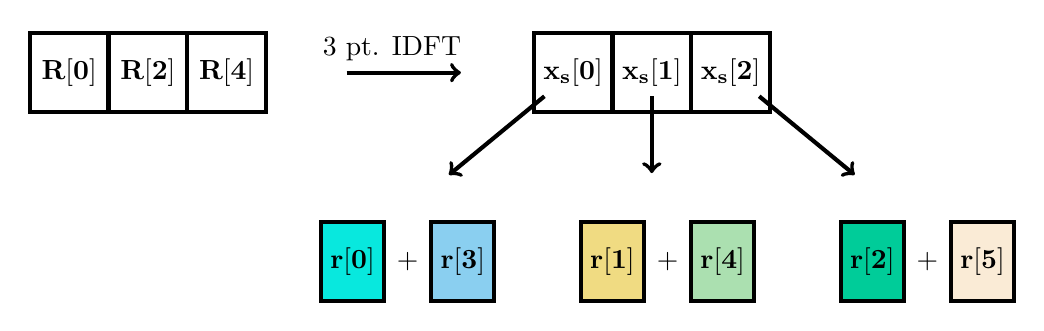
\begin{tikzpicture}

\definecolor{brightturquoise}{rgb}{0.03, 0.91, 0.87}
\definecolor{buff}{rgb}{0.94, 0.86, 0.51}
\definecolor{caribbeangreen}{rgb}{0.0, 0.8, 0.6}
\definecolor{celadon}{rgb}{0.67, 0.88, 0.69}
\definecolor{darktangerine}{rgb}{1.0, 0.66, 0.07}
\definecolor{darkviolet}{rgb}{0.58, 0.0, 0.83}
\definecolor{deepskyblue}{rgb}{0.0, 0.75, 1.0}
\definecolor{amber(sae/ece)}{rgb}{1.0, 0.49, 0.0}
\definecolor{antiquewhite}{rgb}{0.98, 0.92, 0.84}
\definecolor{applegreen}{rgb}{0.55, 0.71, 0.0}
\definecolor{babyblue}{rgb}{0.54, 0.81, 0.94}



% x_{s} (down-sample by 2) 
\draw[thick,line  width =1.5pt]  (3.9,0) rectangle (4.9,-1);
\draw[thick,line  width =1.5pt]  (4.9,0) rectangle (5.9,-1);
\draw[thick,line  width =1.5pt]  (5.9,0) rectangle (6.9,-1);
\node at (4.4,-0.5) {$\bf R[0]$};
\node at (5.4,-0.5) {$\bf R[2]$};
\node at (6.4,-0.5) {$\bf R[4]$};

% DFT arrow
\node (v1) at (7.8,-0.5) {};
\node (v2) at (9.5,-0.5) {};
\draw[thick, ->,line  width =1.5pt]  (v1) edge (v2);
\node at (8.5,-0.2) {3 pt. IDFT};

% X_{s} (DFT of x_{s}) 
\draw[thick,line  width =1.5pt]  (10.3,0) rectangle (11.3,-1);
\draw[thick,line  width =1.5pt]  (11.3,0) rectangle (12.3,-1);
\draw[thick,line  width =1.5pt]  (12.3,0) rectangle (13.3,-1);
\node (v3) at (10.8,-0.5) {$\bf x_{s}[0]$};
\node (v5) at (11.8,-0.5) {$\bf x_{s}[1]$};
\node (v7) at (12.8,-0.5) {$\bf x_{s}[2]$};

\node (v4) at (9.1,-1.9) {};
\node (v6) at (11.8,-1.9) {};
\node (v8) at (14.5,-1.9) {};
\draw[thick,->,line  width =1.5pt]  (v3) edge (v4);
\draw[thick,->,line  width =1.5pt]  (v5) edge (v6);
\draw[thick,->,line  width =1.5pt]  (v7) edge (v8);
\draw[thick,fill=brightturquoise,line  width =1.5pt]  (7.6,-2.4) rectangle (8.4,-3.4);
\draw[thick,fill=babyblue,line  width =1.5pt]  (9,-2.4) rectangle (9.8,-3.4);
\draw[thick,fill=buff,line  width =1.5pt]  (10.9,-2.4) rectangle (11.7,-3.4);
\draw[thick,fill=celadon,line  width =1.5pt]  (12.3,-2.4) rectangle (13.1,-3.4);
\draw[thick,fill=caribbeangreen,line  width =1.5pt]  (14.2,-2.4) rectangle (15,-3.4);
\draw[thick,fill=antiquewhite,line  width =1.5pt]  (15.6,-2.4) rectangle (16.4,-3.4);


\node at (8,-2.9) {$\mathbf{r[0]}$};
\node at (9.4,-2.9) {$\bf r[3]$};
\node at (8.7,-2.9) {$\mathbf{+}$};

\node at (11.3,-2.9) {$\bf r[1]$};
\node at (12.7,-2.9) {$\bf r[4]$};
\node at (15.3,-2.9) {$\mathbf{+}$};

\node at (14.6,-2.9) {$\bf r[2]$};
\node at (16,-2.9) {$\bf r[5]$};
\node at (12,-2.9) {$\mathbf{+}$};
\end{tikzpicture}